\section{Introdução}
\label{sec:manual}

Seja muito bem vindo ao manual do usuário do Grata (Gerenciador de Reuniões e Atas), a ferramenta que irá te ajudar você, caro gerente de projetos, a melhorar suas reuniões.

Este \textit{software} foi desenvolvida para ser uma ferramenta completamente gratuita, com código aberto, e que permite uma custumização das empresas para seus problemas especifícos. Tudo relacionado podem ser encontrados nos seguintes links: \href{https://github.com/FGAProjects/TCC}{TCC}, \href{https://github.com/MrVictor42/Grata-Backend-v2}{Backend}, e \href{https://github.com/MrVictor42/Grata-Frontend-v2}{Frontend}. 

\textbf{Em caso de qualquer dúvida, pertinentes a este projeto, por favor entrar em contato com o desenvolvedor deste projeto pelo email: mrvictor042@gmail.com.}

\textbf{A ferramenta foi desenvolvida para ser gratuita e adaptável as necessidades das empresas, e a custumização de novas funcionalidades, servidores, banco de dados e qualquer coisa além do desenvolvido neste projeto, ficará a cargo da empresa.}

\section{Instalação}

O Grata é uma ferramenta online, não necessitando de instalação, contudo para que seja realizada alterações no mesmo deve ser realizado via código. Pedimos que qualquer desejo de mudança na ferramenta, seja realizada a partir de um \textit{"fork"} nos repositórios do \textit{Github}, linkados acima.

Para ajudar no desenvolvimento de novas funcionalidades, ou ainda alterações no formato original do Grata, todos os códigos relacionados a ferramenta foram implementados utilizando o \textit{Docker}. A seguir, como instalar e utilizar o \textit{Docker} do projeto:

\subsection{Windows}

\subsubsection{Docker}

Para instalar o \textit{Docker} no sistema operacional \textit{Windows}, basta seguir os passos do link a seguir: \href{https://docs.docker.com/docker-for-windows/install/}{Docker-Windows}.

\subsection{Ubuntu}

\subsubsection{Docker}

Para instalar o \textit{Docker} no sistema operacional \textit{Ubuntu} e suas derivações, basta seguir os passos do link a seguir: \href{https://www.digitalocean.com/community/tutorials/how-to-install-and-use-docker-on-ubuntu-20-04}{Docker-Ubuntu}.

\subsubsection{Docker-Compose}

Para instalar o \textit{Docker-Compose} no sistema operacional \textit{Ubuntu} e suas derivações, basta seguir os passos do link a seguir: \href{https://www.digitalocean.com/community/tutorials/how-to-install-and-use-docker-compose-on-ubuntu-20-04-pt}{Docker-Compose-Ubuntu}.

No sistema operacional \textit{Ubuntu} e suas derivações, em ambas os projetos (\textit{frontend/backend}), devem ser rodado os seguintes comandos: 
\begin{itemize}
    \item docker-compose build (Para criar a build do projeto);
    \item docker-compose up (Para rodar o projeto).
\end{itemize}

\section{Informações Importantes}

O Grata foi construido seguindo o modelo do caso de estudo, como explicado no tópico \ref{sec:caso_de_estudo}. Desta maneira, para existir uma reunião, deve existir um projeto e um projeto está relacionado diretamente ao setor. Existe então uma questão de dependência.

Os administradores podem visualizar mais informações que os participantes, bem como poder editar e excluir coisas que os participantes não podem. Em todo caso, caso algum administrador deseja excluir um setor, que já possui projetos em andamento, será lançada uma mensagem para confirmação da ação, como meio de tentar impedir uma ação erronea.

Todas as informações podem ser inseridas e alteradas, salvo as de reuniões com o status de "Finalizada". Em alguns momentos, pode ser necessário dá um "\textit{refresh}" na página, para atualizar as informações, isso pode acontecer nos processos de edição e exclusão de algo.

\section{Como Utilizar?}

\subsection{Tela Inicial e Login}

\begin{figure}[H]
    \centering
    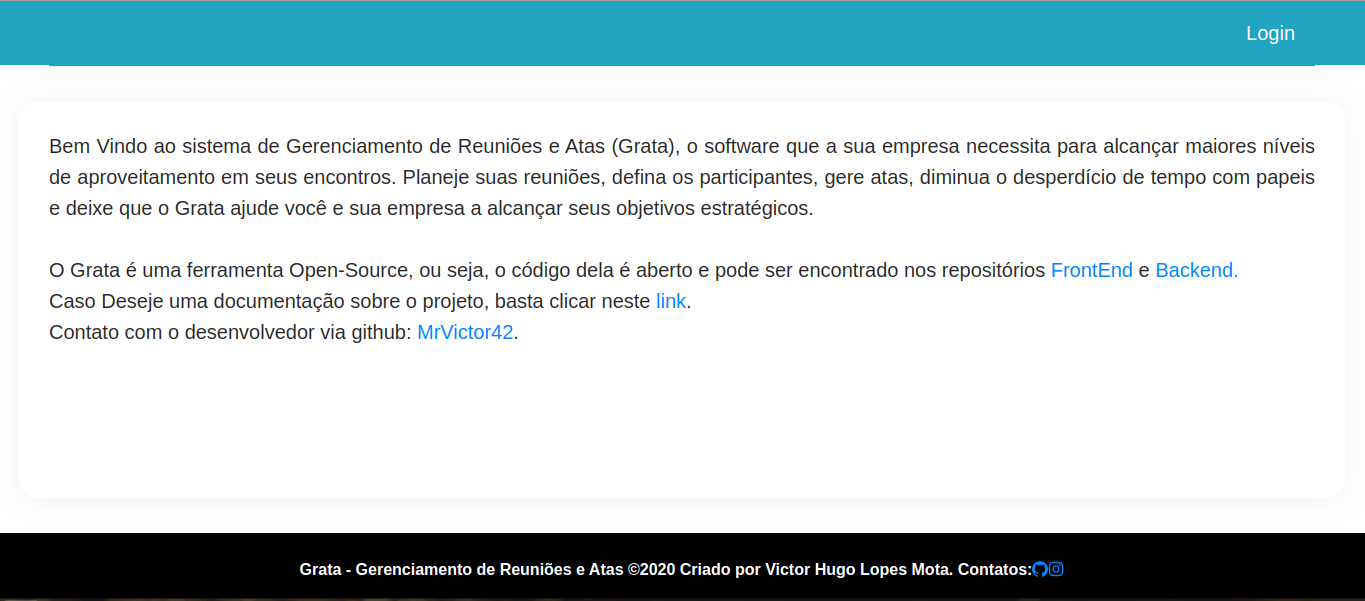
\includegraphics[width=1.0\textwidth]{figuras/tela_inicial.png}
    \caption{Tela Inicial. Fonte: Própria}
    \label{img:tela_inicial}
\end{figure}

A imagem \ref{img:tela_inicial}, mostra a tela inicial da ferramenta, com uma rápida explicação sobre o que é o \textit{software} em questão. Para começar a acessar os recursos da ferramenta, basta clicar em "\textit{Login}".

\begin{figure}[H]
    \centering
    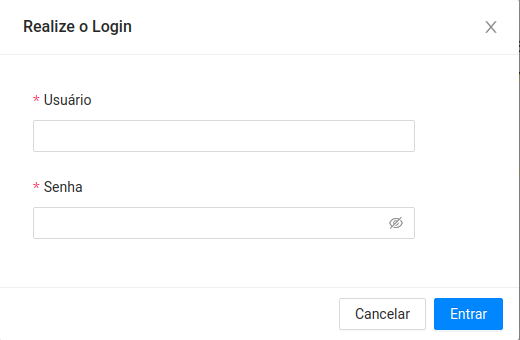
\includegraphics[width=1.0\textwidth]{figuras/tela_login.png}
    \caption{Login. Fonte: Própria}
    \label{img:tela_login}
\end{figure}

Inserindo suas credenciais na ferramenta, você poderá acessar adequeadamente as funções do sistema.

\textbf{No primeiro acesso na ferramenta, entre em contato com o desenvolvedor.}

\subsection{Perfis de Usuários}

Os usuários no Grata são divididos em dois grupos: Administrador e Participante da Reunião.

O \textbf{Administrador}, é aquele que tem as maiores liberdades dentro do sistema, podendo adicionar novos usuários, criar setores, gerencia reuniões, comentar nas reuniões, e é ele que prove os insumos para uma reunião. Este perfil também pode excluir usuários do sistema e alterar as permissões dos demais usuários, ou seja, ele pode transformar um partipante da reunião em um administrador.

O \textbf{Participante}, é aquele que deve ser convidado pelo administrador a compor uma reunião, além de poder comentar sobre a mesma e estar por dentro do que rumo dos projetos em que está participando.

\subsection{Usuários}

\begin{figure}[H]
    \centering
    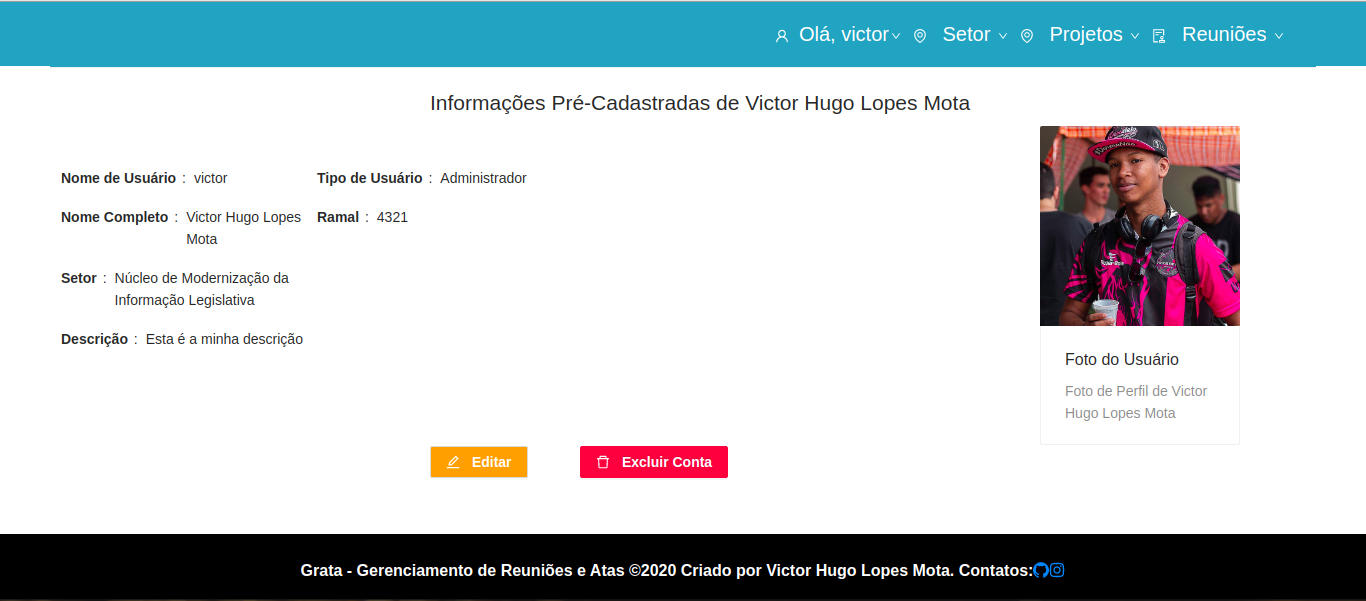
\includegraphics[width=1.0\textwidth]{figuras/tela_perfil.png}
    \caption{Tela de Perfil do Usuário. Fonte: Própria}
    \label{img:tela_perfil_usuario}
\end{figure}

A imagem \ref{img:tela_perfil_usuario}, mostra a tela de perfil de usuário qualquer, contendo suas informações básicas. Todos os usuários podem editar suas informações, além de colocar o setor em que trabalham.

Ao clicar no botão "Editar", o sistema irá mostrar a seguinte tela:

\begin{figure}[H]
    \centering
    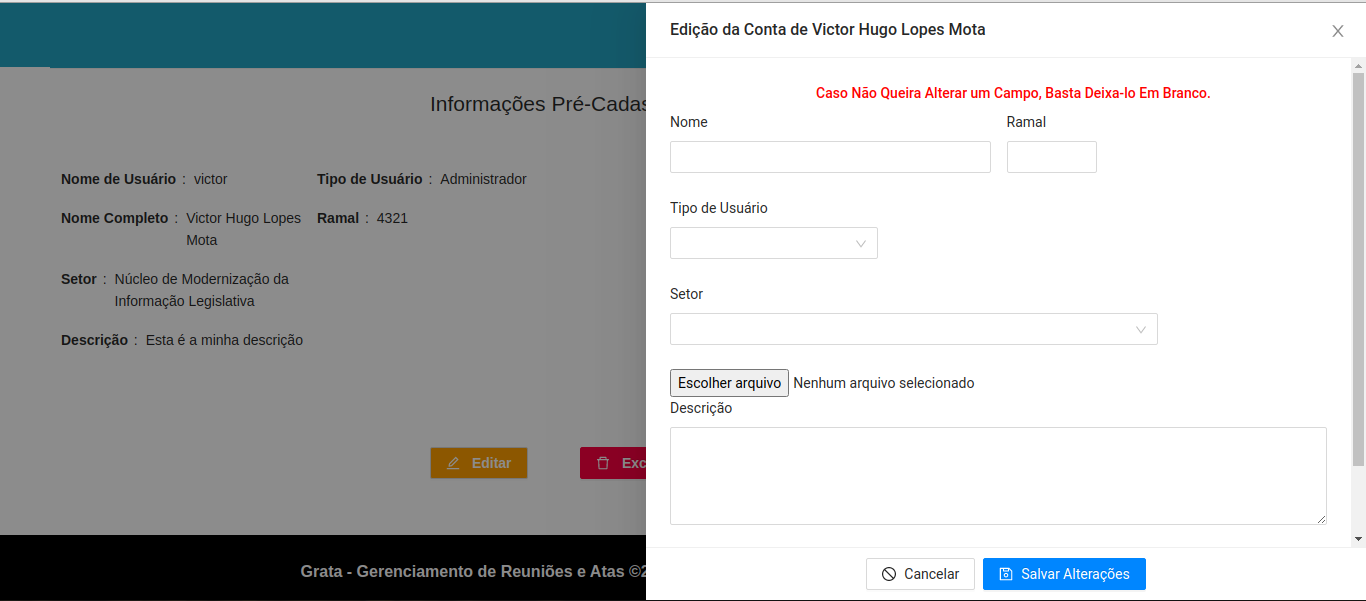
\includegraphics[width=1.0\textwidth]{figuras/edicao_usuario.png}
    \caption{Tela de Edição do Usuário. Fonte: Própria}
    \label{img:tela_edicao_usuario}
\end{figure}

Na tela da imagem \ref{img:tela_edicao_usuario}, mostra os campos que podem ser alterados pelo usuário (Administrador). Os participantes de usuários a partir do processo de edição, podem alterar informações previamente incluidas pelo administrador.

\subsection{Lista de Usuários}

\begin{figure}[H]
    \centering
    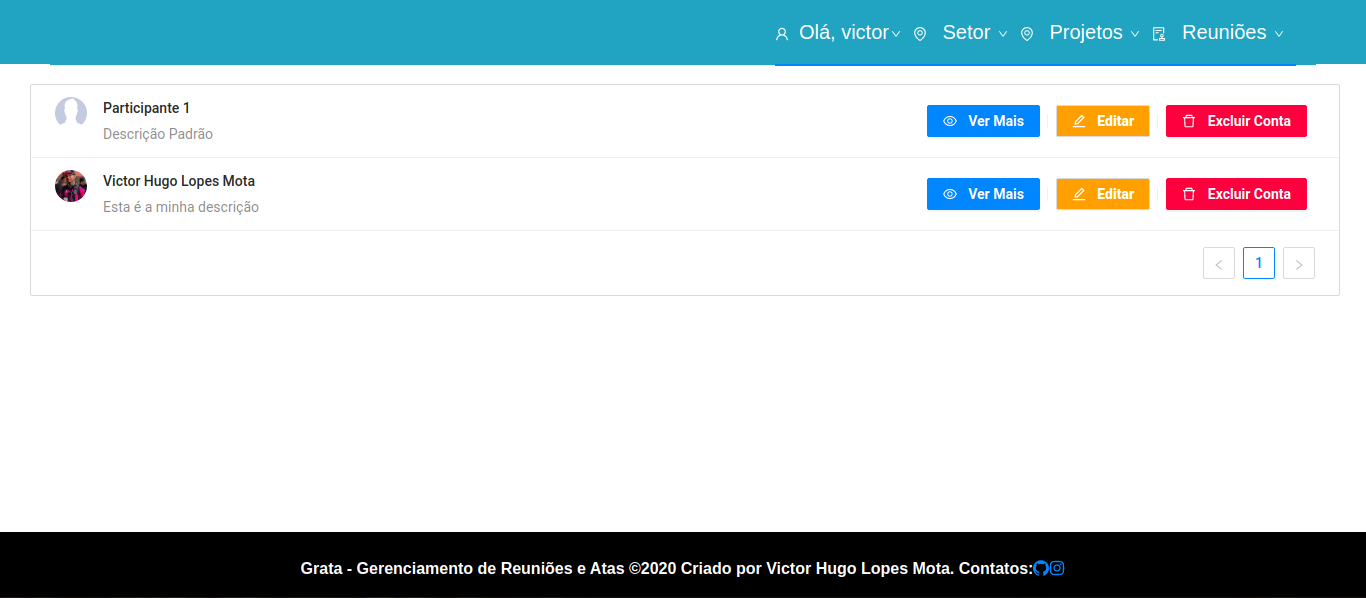
\includegraphics[width=1.0\textwidth]{figuras/lista_de_usuarios.png}
    \caption{Lista de Usuários. Fonte: Própria}
    \label{img:lista_de_usuarios}
\end{figure}

A imagem \ref{img:lista_de_usuarios}, mostra os usuários cadastrados no sistema, mostrando as informações básicas sobre os mesmos. Ao clicar no botão "Ver Mais", é possível visualizar os projetos em que eles estão trabalhando e as reuniões que estão participando. Isso é mostrado na imagem \ref{img:ver_mais}:

\begin{figure}[H]
    \centering
    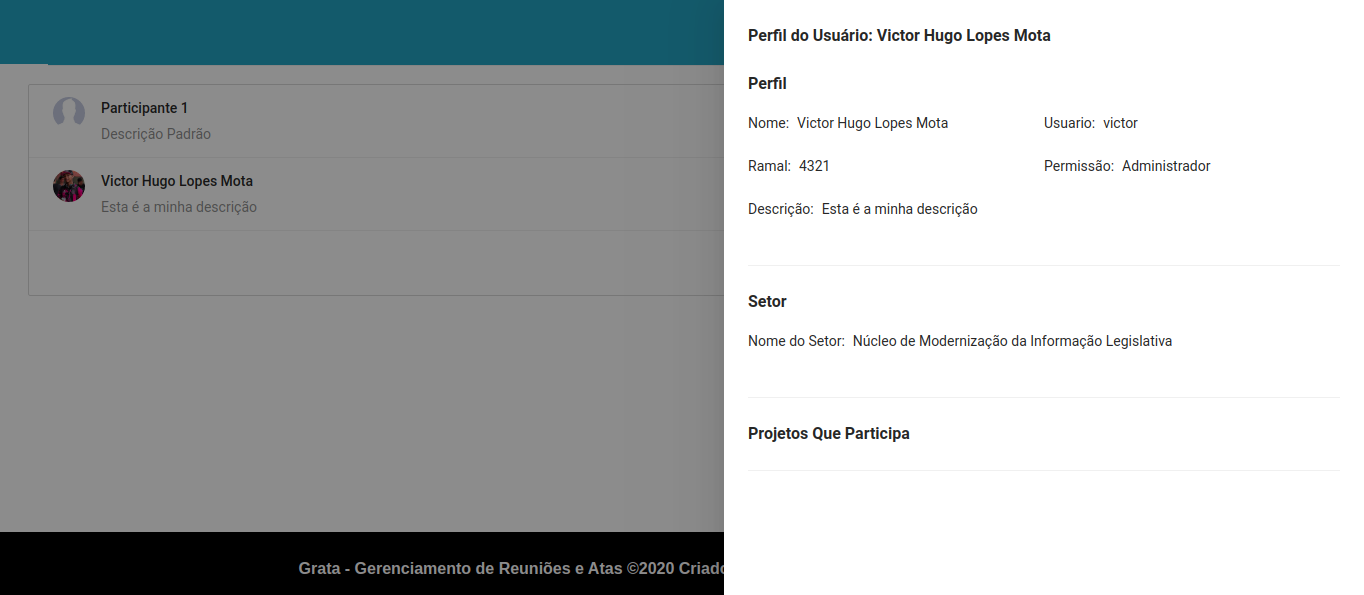
\includegraphics[width=1.0\textwidth]{figuras/ver_mais_usuarios.png}
    \caption{Ver Mais Usuários. Fonte: Própria}
    \label{img:ver_mais}
\end{figure}

\subsection{Navbar}

A \textit{Navbar} do projeto é diferente para os tipos de usuários, mas em todos os casos, ao passar o \textit{mouse} sobre um item da \textit{Navbar}, uma pequena lista de itens irá aparecer e será clicável.

\subsection{Setores}

\subsubsection{Criação de um Setor}

A imagem \ref{img:criacao_de_setor}, mostra os campos que devem ser preenchidos para criar um setor na ferramenta. \textbf{Obs: apenas os administradores podem criar setores.}

\begin{figure}[H]
    \centering
    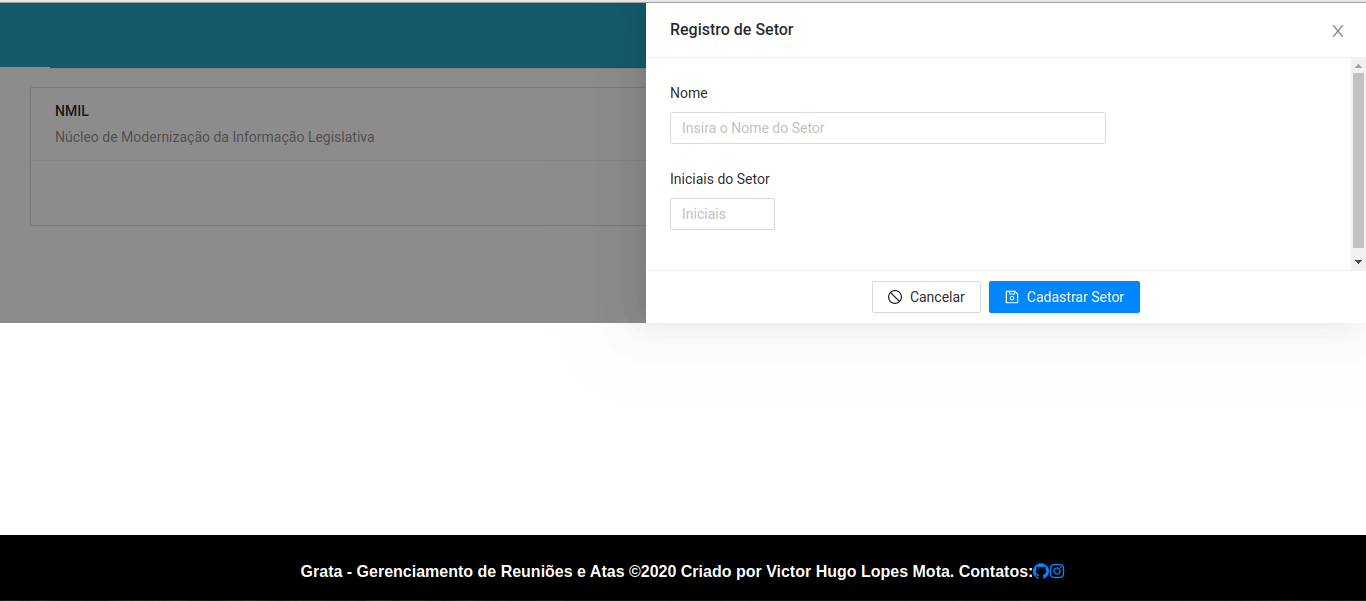
\includegraphics[width=1.0\textwidth]{figuras/criar_setor.png}
    \caption{Criar Setor. Fonte: Própria}
    \label{img:criacao_de_setor}
\end{figure}

\subsubsection{Lista de Setores}

\begin{figure}[H]
    \centering
    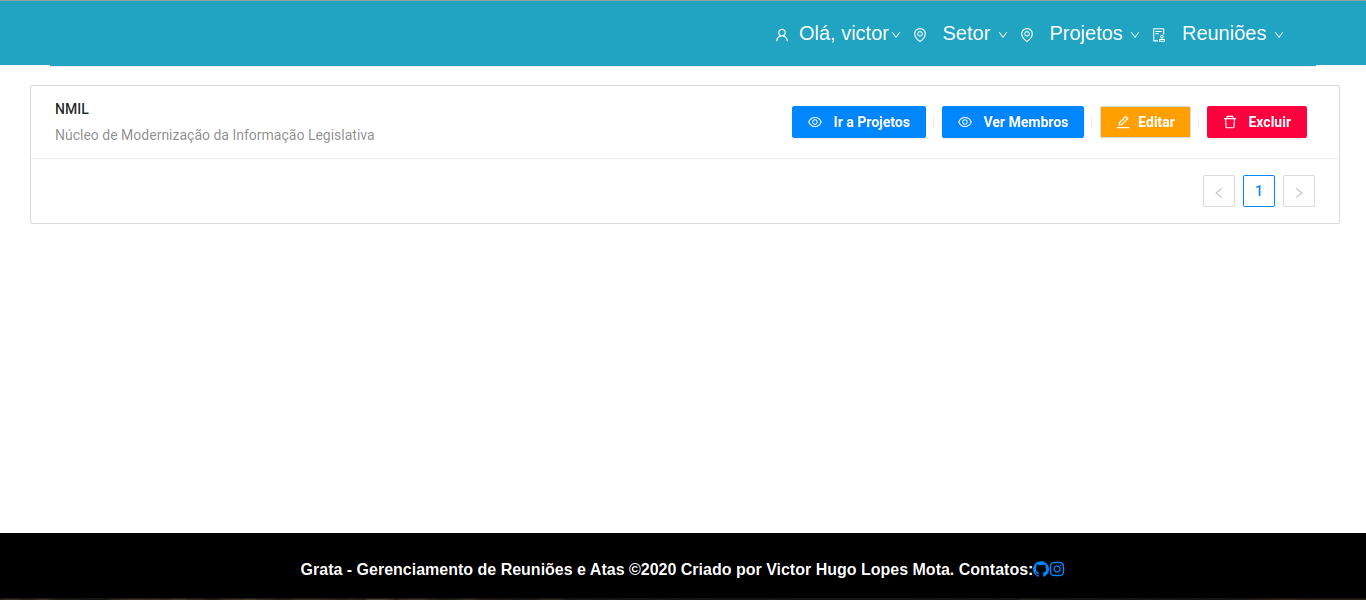
\includegraphics[width=1.0\textwidth]{figuras/lista_de_setores.png}
    \caption{Lista de Setores. Fonte: Própria}
    \label{img:lista_de_setores}
\end{figure}

A lista de setores podem ser vistas por todos os usuários registrados no projeto. Nesta lista, é possível visualizar os projetos e os membros do setor, como mostrado na imagem \ref{img:ver_membros_setores}:

\begin{figure}[H]
    \centering
    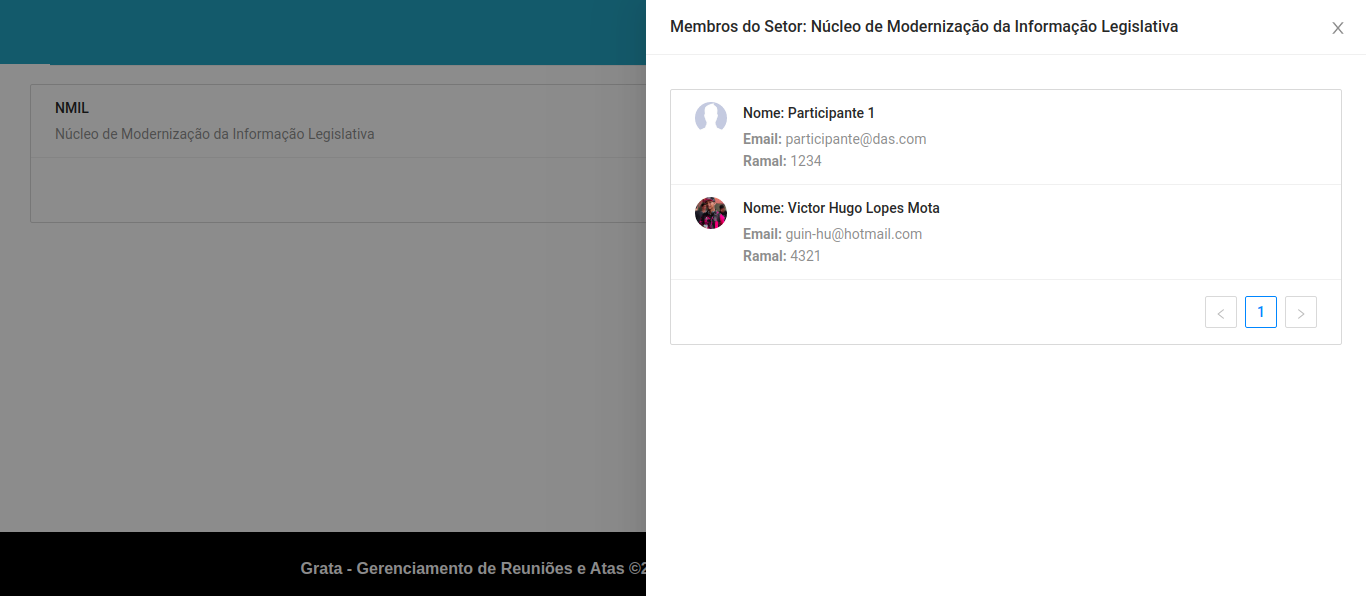
\includegraphics[width=1.0\textwidth]{figuras/membros_setores.png}
    \caption{Ver Membros do Setor. Fonte: Própria}
    \label{img:ver_membros_setores}
\end{figure}

\subsection{Projetos}

\textbf{Todos os membros da ferramenta podem visualizar o andamento dos projetos, contudo, os que gerenciar os projetos são os administradores.}

\subsubsection{Criação de Projetos}

\begin{figure}[H]
    \centering
    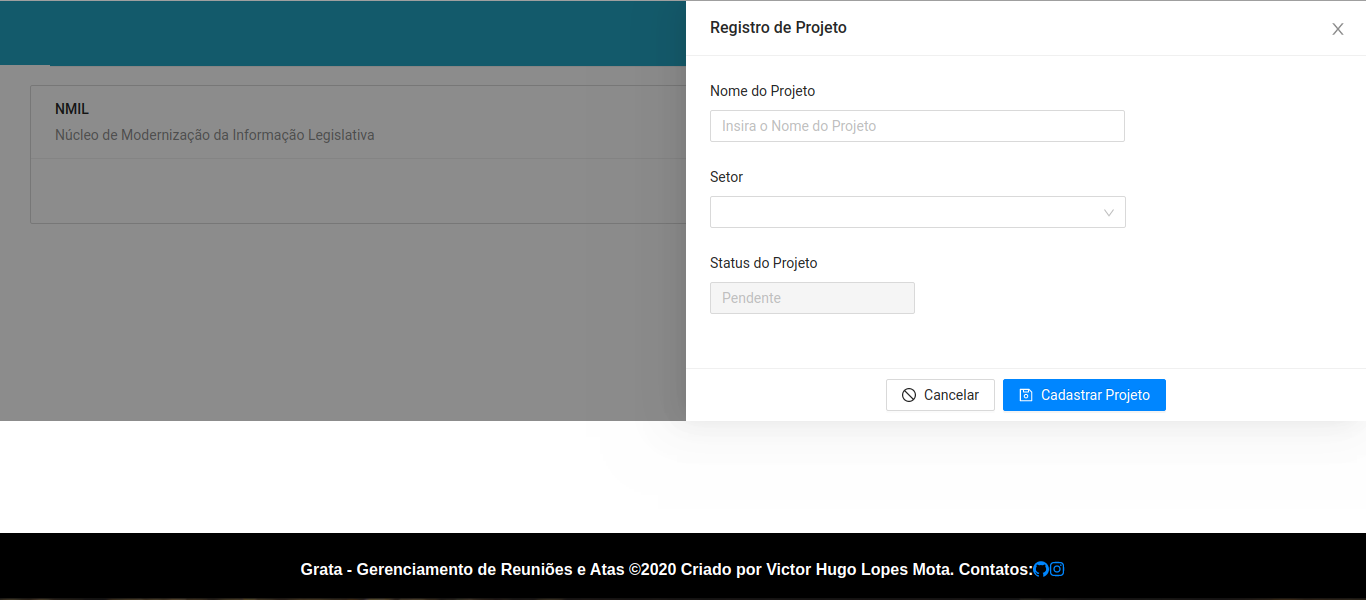
\includegraphics[width=1.0\textwidth]{figuras/criar_projeto.png}
    \caption{Criar Projeto. Fonte: Própria}
    \label{img:criacao_de_projeto}
\end{figure}

\subsubsection{Lista de Projetos}

Os projetos são ligados aos setores, sendo somente acessíveis ao acessar o setor. Um projeto pode possuir uma ou várias reuniões, contudo uma reunião está ligada a apenas um projeto, sendo assim uma relação 1:N.

Um projeto recém criado, começa com o status "Pendente", sendo que o administrador pode mudar esse status apenas "Cancelada". O administrador pode adicionar membros aos projetos, bem como remove-los. Pode visualizar os membros do projeto. Esse ponto é importante, pois os membros que irão compor à reunião, devem ser adicionados antes ao projeto.

\begin{figure}[H]
    \centering
    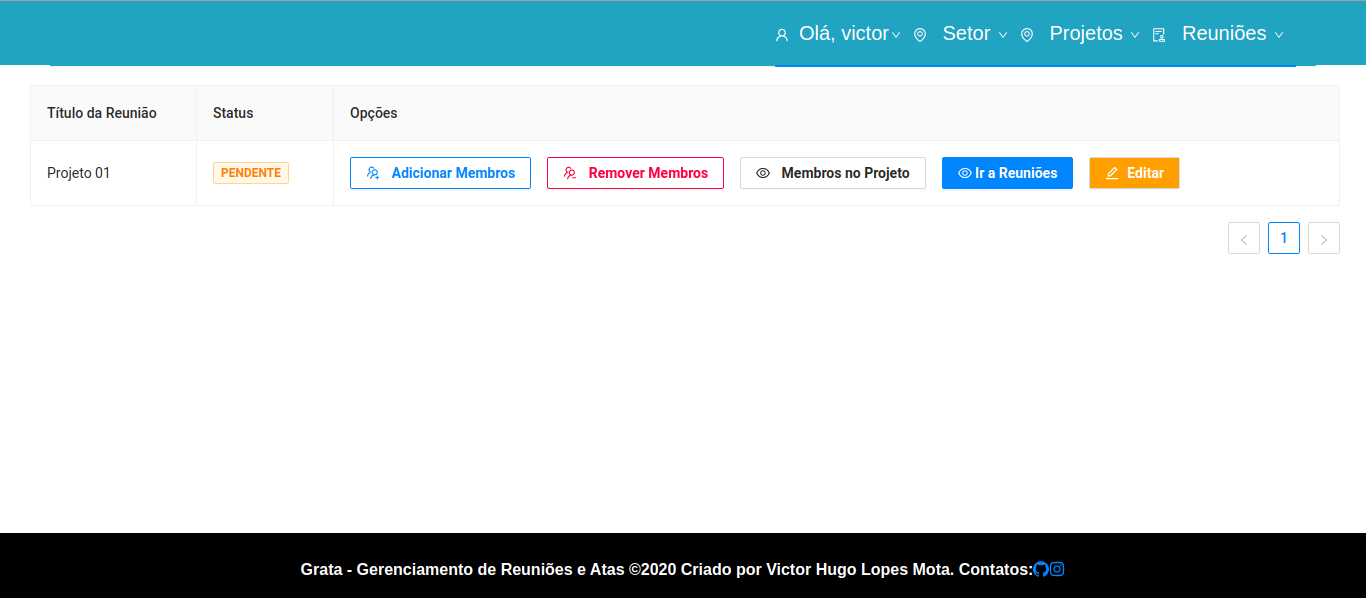
\includegraphics[width=1.0\textwidth]{figuras/lista_de_projetos.png}
    \caption{Lista de Projetos. Fonte: Própria}
    \label{img:lista_de_projetos}
\end{figure}

\subsubsection{Adicionando, Removendo e Visualizando Membros do Projeto}

\begin{figure}[H]
    \centering
    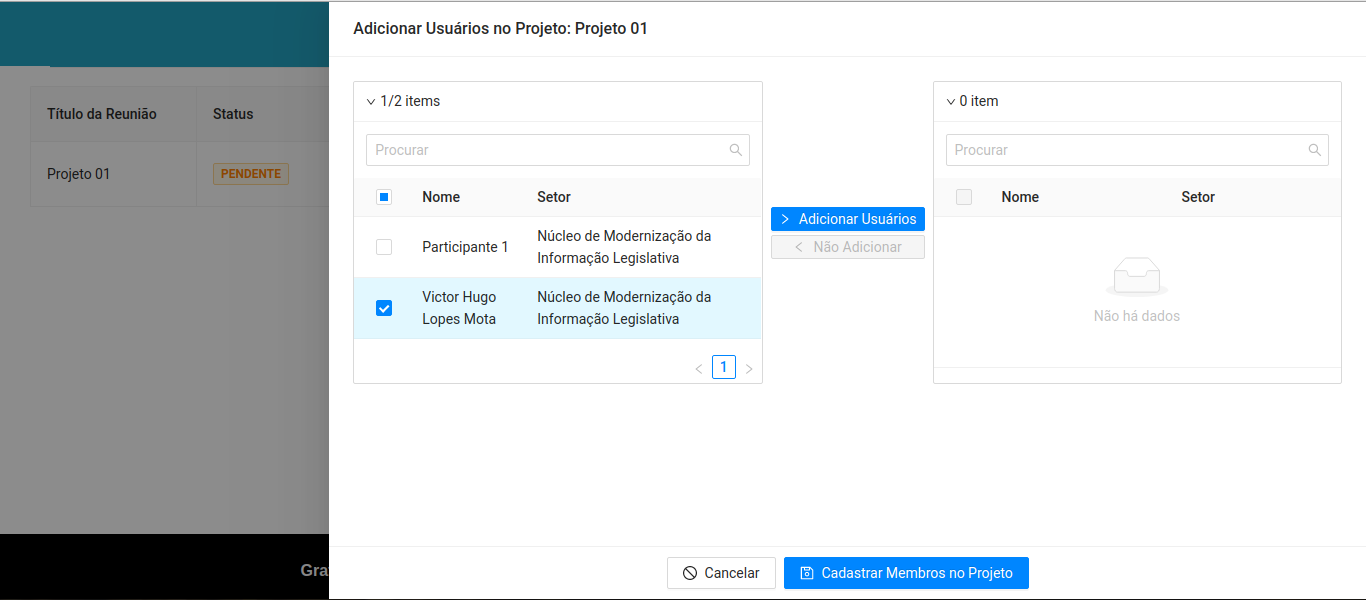
\includegraphics[width=1.0\textwidth]{figuras/adicionando_membros_projeto.png}
    \caption{Adicionar Membros ao Projeto. Fonte: Própria}
    \label{img:adicionar_membros_projeto}
\end{figure}

\begin{figure}[H]
    \centering
    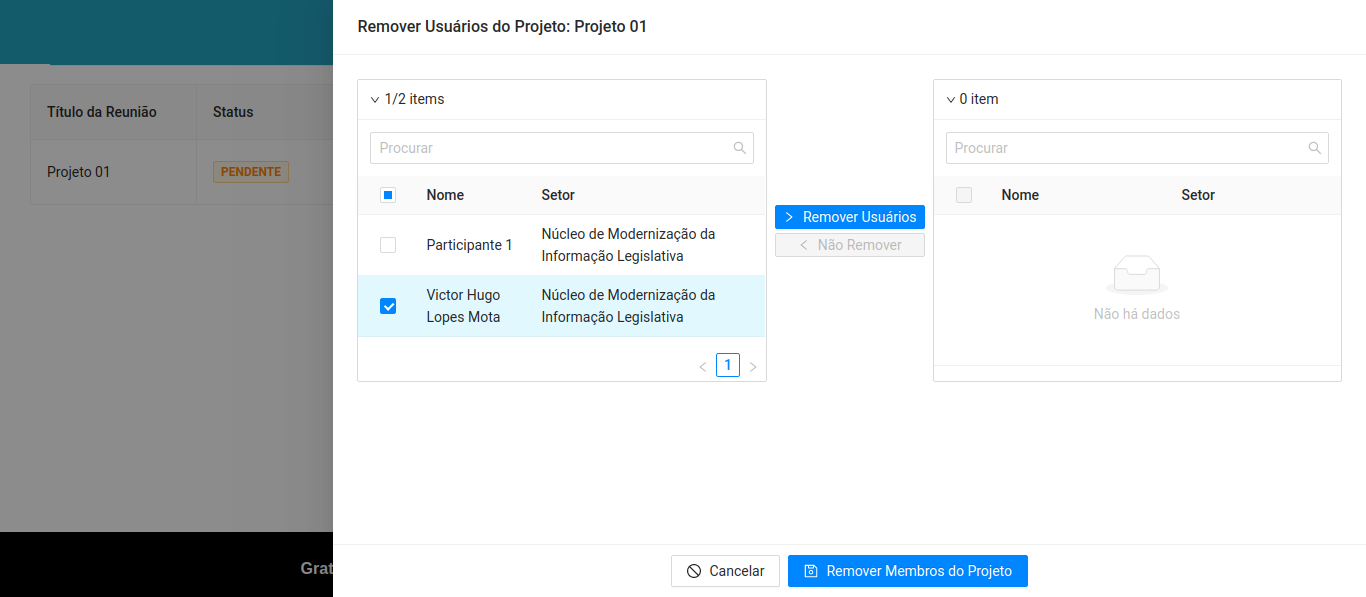
\includegraphics[width=1.0\textwidth]{figuras/remover_usuarios_projeto.png}
    \caption{Remover Membros do Projetos. Fonte: Própria}
    \label{img:remover_membros_projeto}
\end{figure}

\begin{figure}[H]
    \centering
    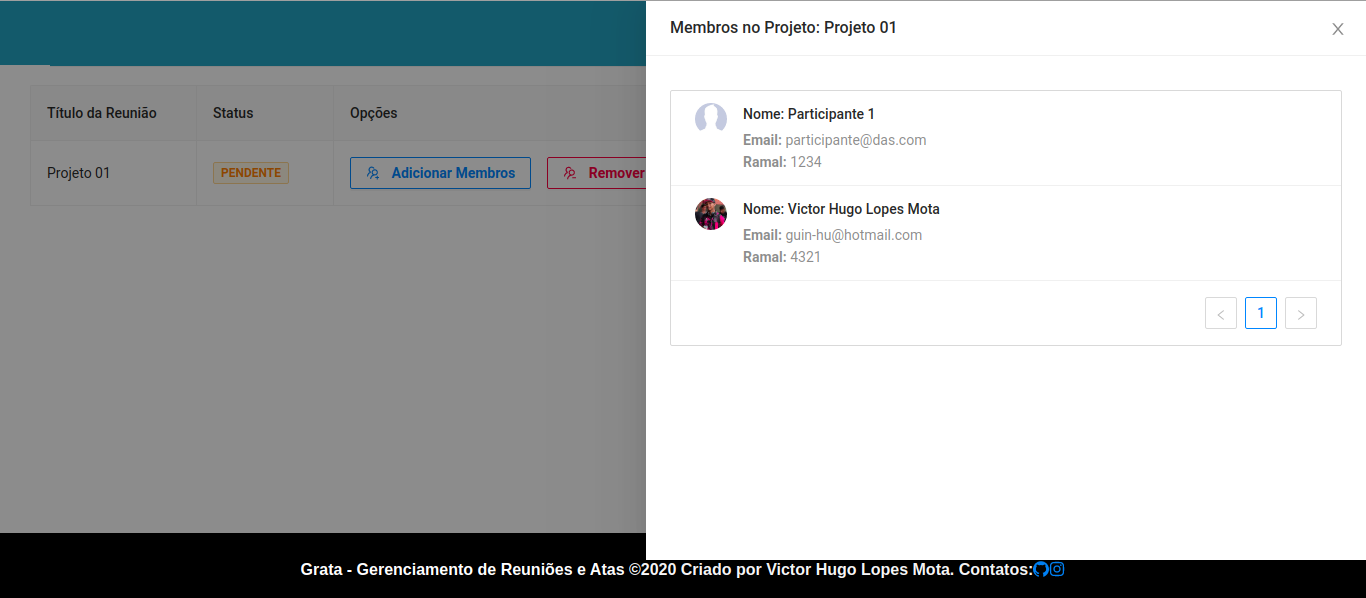
\includegraphics[width=1.0\textwidth]{figuras/membros_do_projeto.png}
    \caption{Membros do Projetos. Fonte: Própria}
    \label{img:membros_da_reuniao}
\end{figure}

\subsection{Reuniões}

\subsubsection{Criar Reuniões}

As reuniões só podem ser criadas depois de um projeto e eles devem ser associados. Os tópicos devem ser preenchidos, e toda reunião deve ter um líder, bem como data e horário pré-definidos. 

\begin{figure}[H]
    \centering
    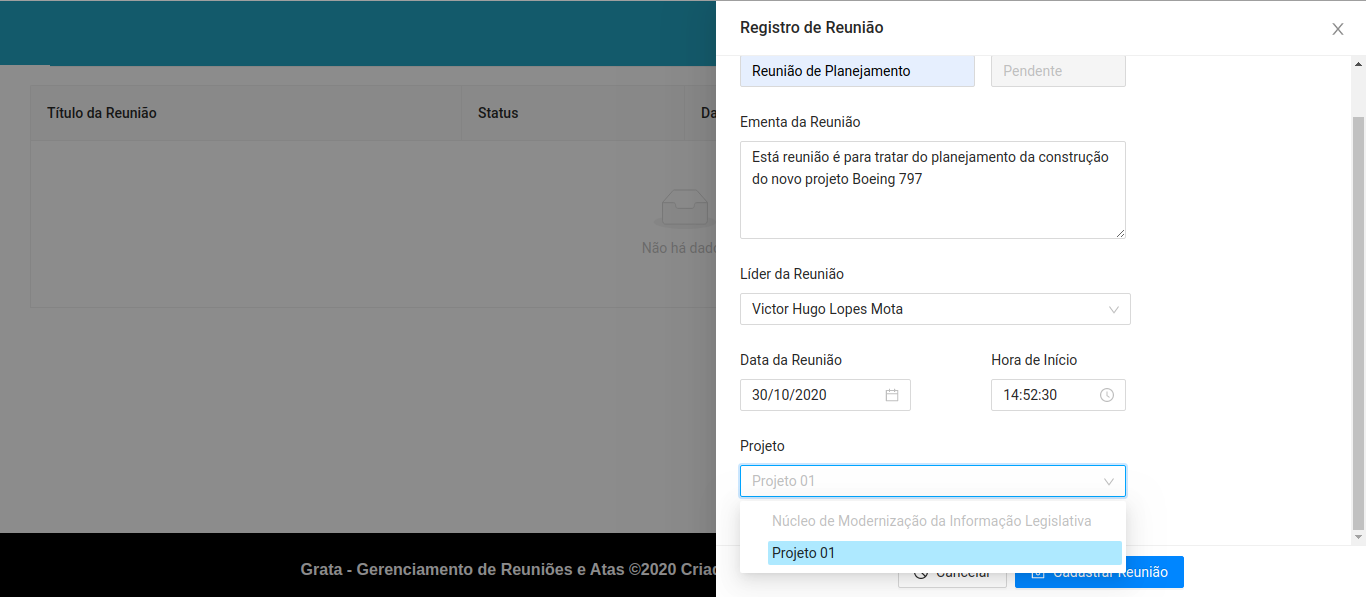
\includegraphics[width=1.0\textwidth]{figuras/criar_reuniao.png}
    \caption{Criar Reunião. Fonte: Própria}
    \label{img:criar_reuniao}
\end{figure}

\subsubsection{Lista de Reuniões}

Dentro dos projetos, ficam as reuniões associadas a eles. Todas as reuniões inicialmente começam com o status pendente, como pode ser visto na imagem \ref{img:lista_de_reunioes}:

\begin{figure}[H]
    \centering
    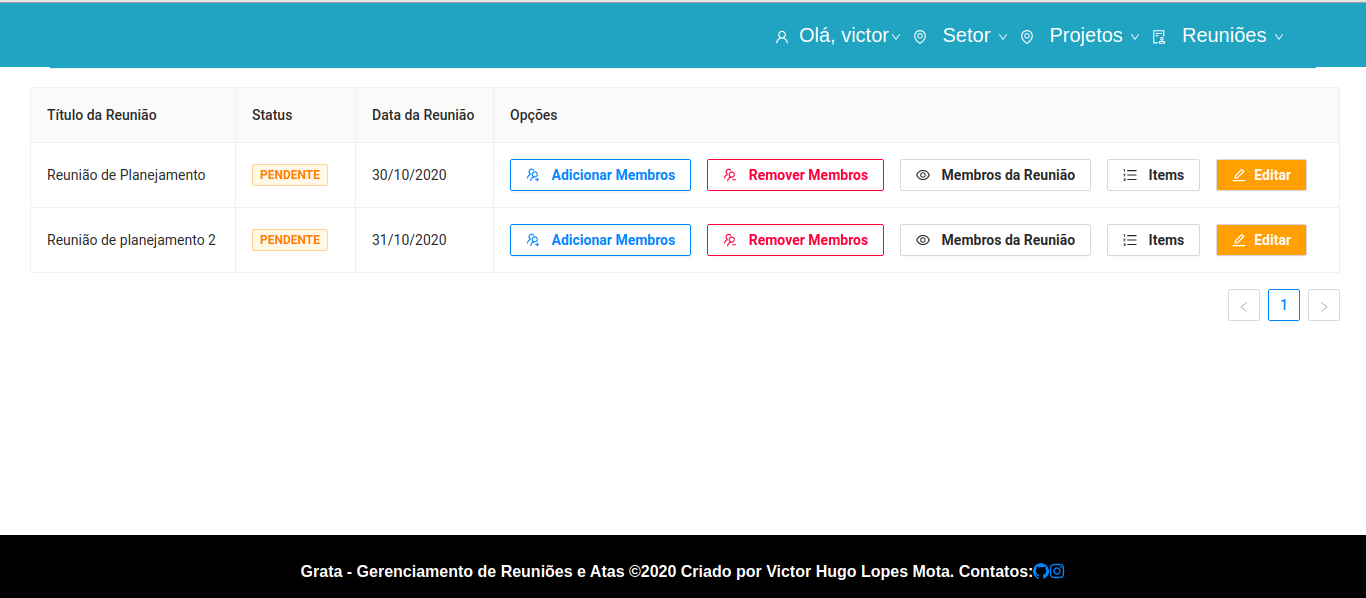
\includegraphics[width=1.0\textwidth]{figuras/lista_reunioes.png}
    \caption{Lista de Reuniões. Fonte: Própria}
    \label{img:lista_de_reunioes}
\end{figure}

\subsubsection{Adicionar, Removendo e Visualizando Membros da Reunião}

\begin{figure}[H]
    \centering
    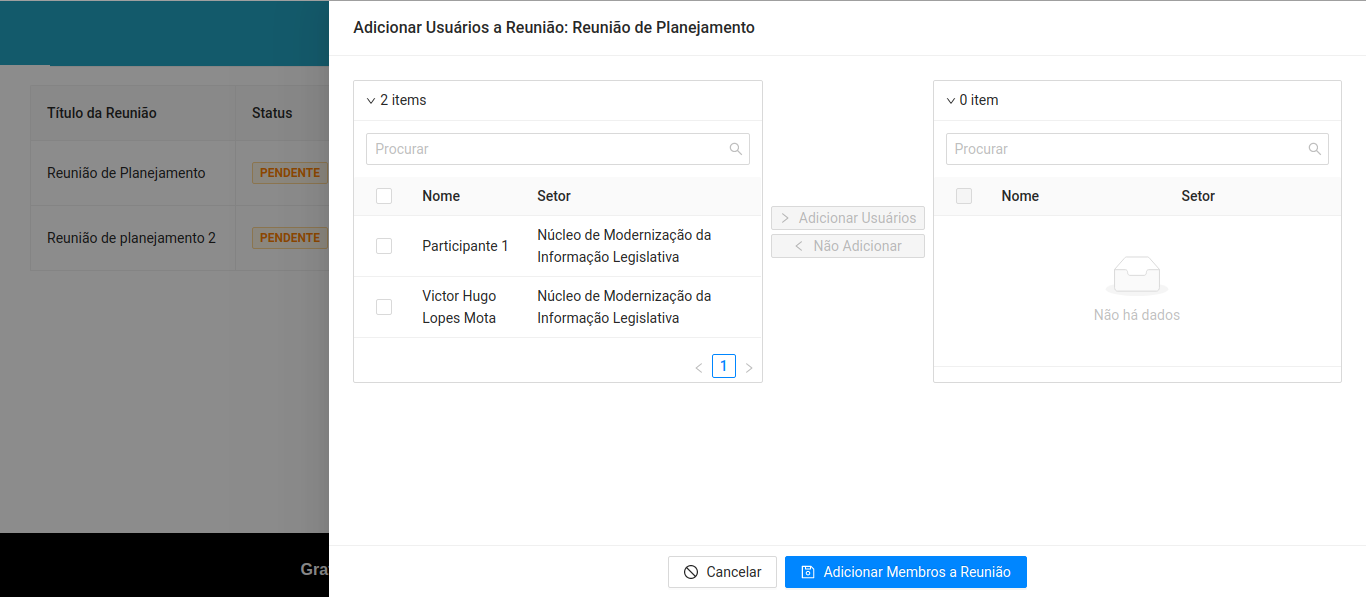
\includegraphics[width=1.0\textwidth]{figuras/adicionando_membros_reuniao.png}
    \caption{Adicionando Membros à Reunião. Fonte: Própria}
    \label{img:adicionar_membros_a_reuniao}
\end{figure}

\begin{figure}[H]
    \centering
    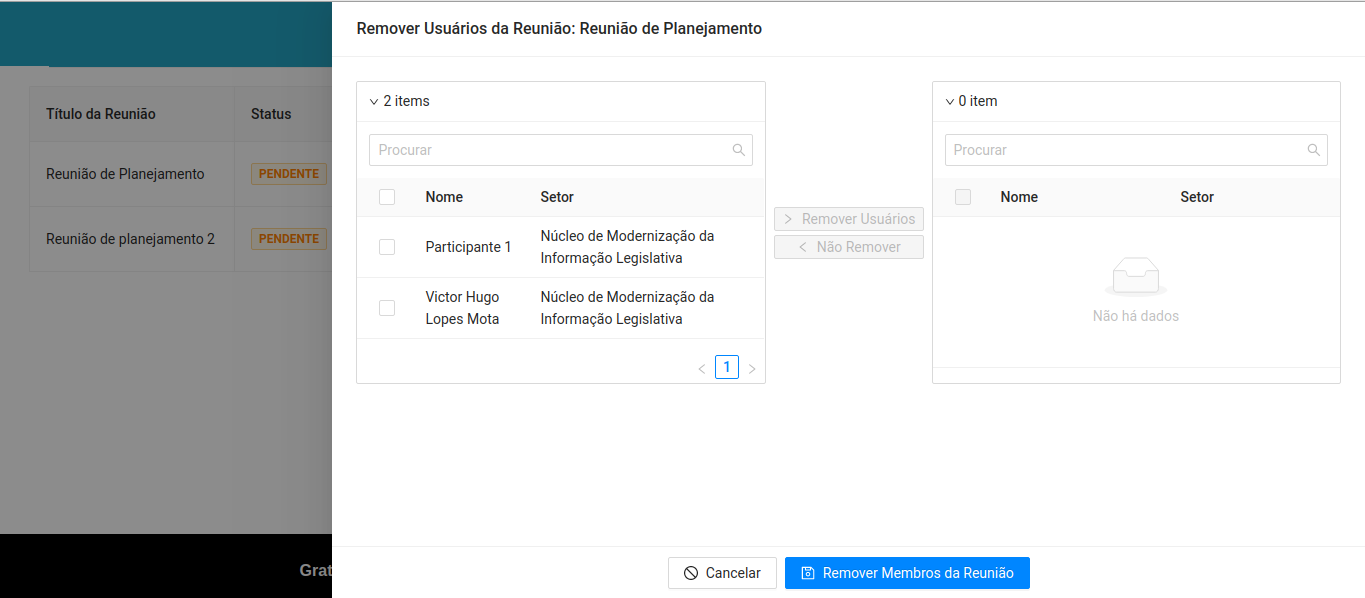
\includegraphics[width=1.0\textwidth]{figuras/remover_usuarios_reuniao.png}
    \caption{Removendo Membros da Reunião. Fonte: Própria}
    \label{img:remover_membros_a_reuniao}
\end{figure}

\begin{figure}[H]
    \centering
    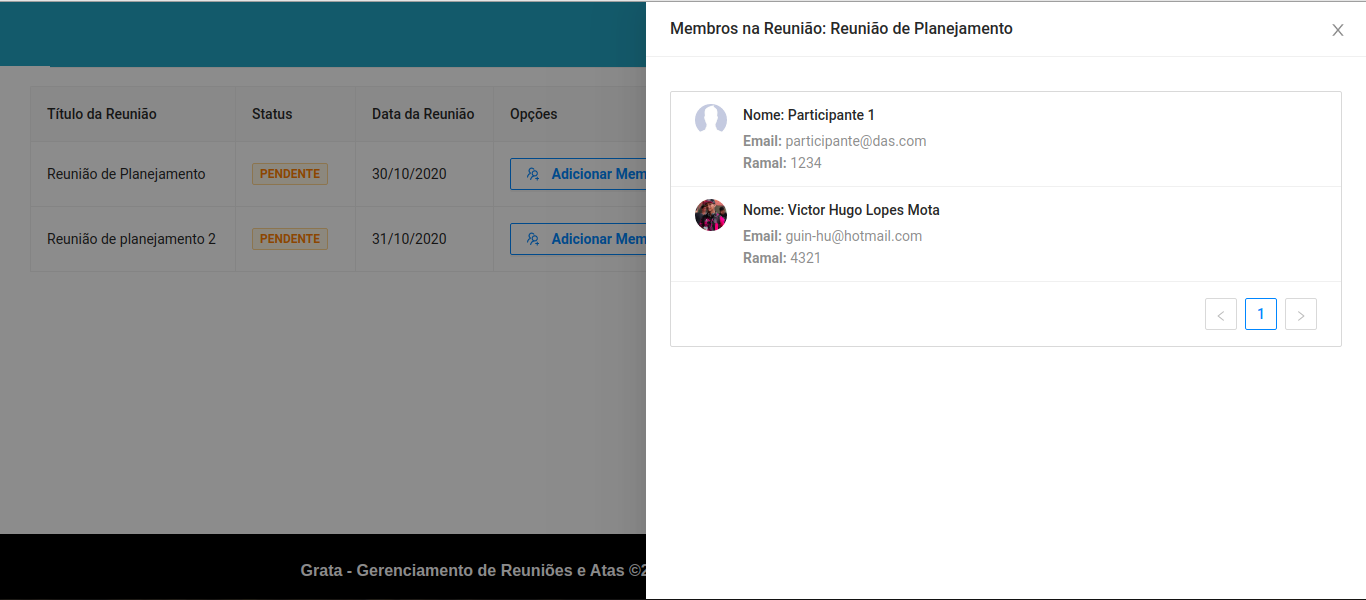
\includegraphics[width=1.0\textwidth]{figuras/membros_da_reuniao.png}
    \caption{Lista de Membros da Reunião. Fonte: Própria}
    \label{img:membros_da_reuniao}
\end{figure}

\subsubsection{Itens da Reunião}

Nos itens da reunião, são definidas as regras da reunião e os tópicos. Este é o último ponto do processo antes do status da reunião ser alterado para "Agendada".

\begin{figure}[H]
    \centering
    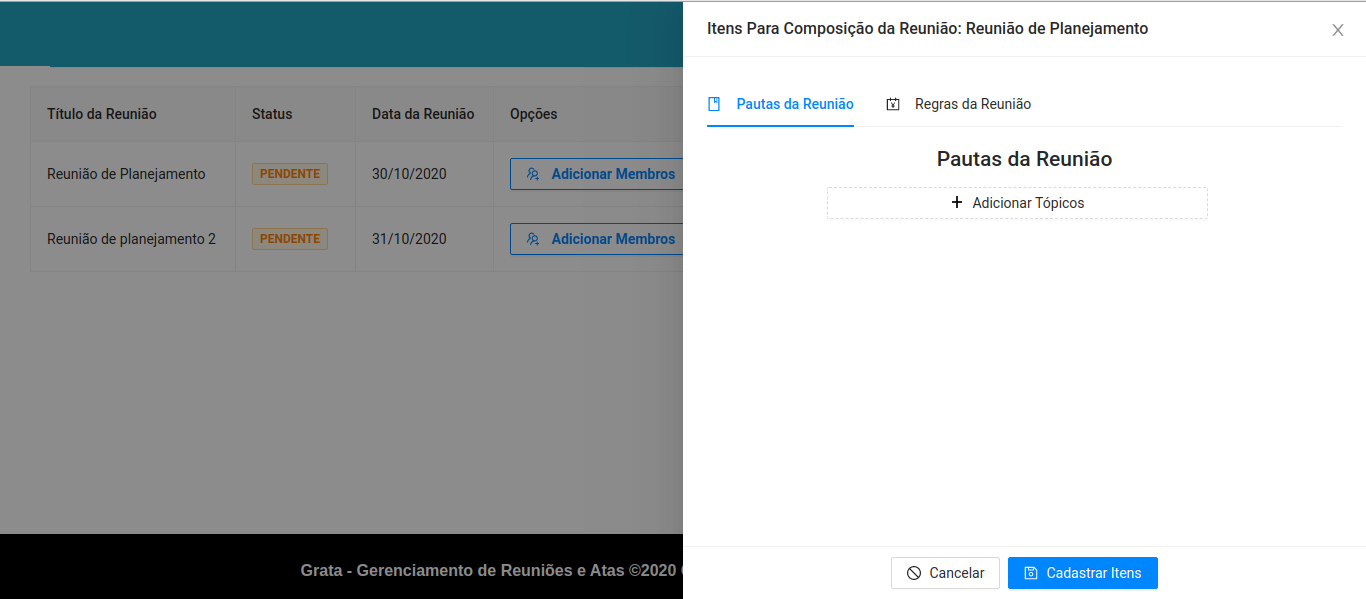
\includegraphics[width=1.0\textwidth]{figuras/itens_reuniao.png}
    \caption{Itens da Reunião. Fonte: Própria}
    \label{img:itens_da_reuniao}
\end{figure}

\begin{figure}[H]
    \centering
    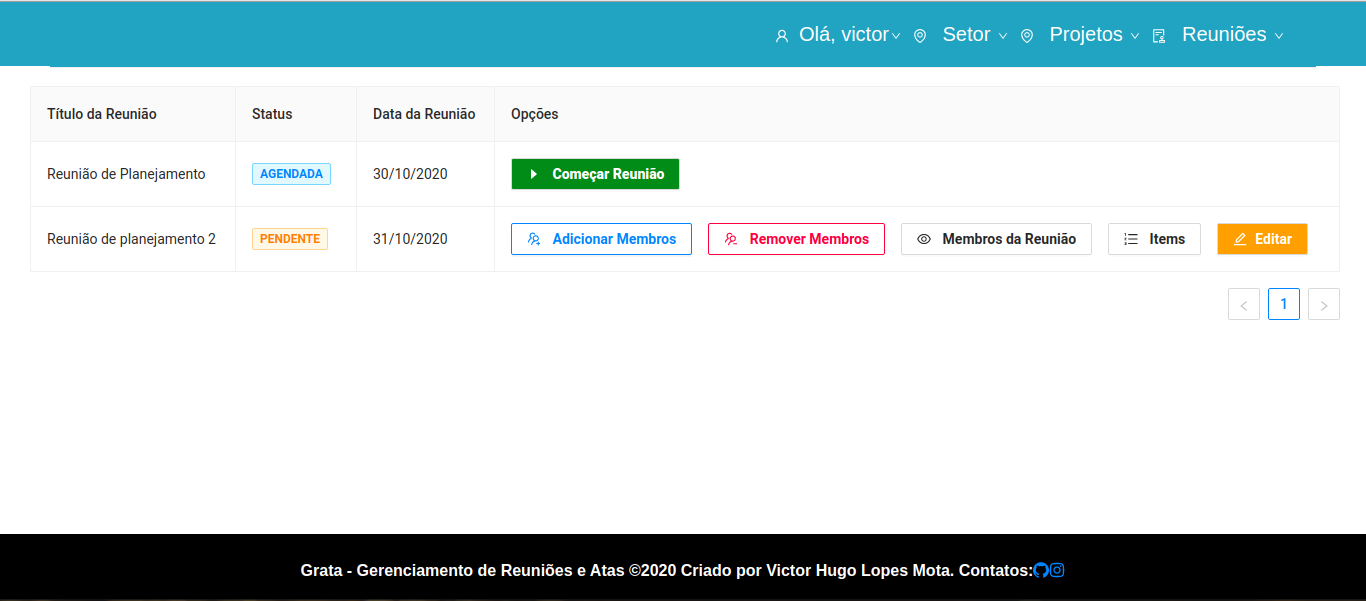
\includegraphics[width=1.0\textwidth]{figuras/reuniao_agendada.png}
    \caption{Reunião Agendada. Fonte: Própria}
    \label{img:itens_da_reuniao}
\end{figure}

Quando a reunião muda para o status de "Agendada", não se pode mais alterar os dados nela.

\subsubsection{Reunião Agendada}

Com a reunião agendada, o gerente pode clicar no botão "Começar a Reunião". O sistema irá para a página da imagem \ref{img:informacoes_reuniao}:

\begin{figure}[H]
    \centering
    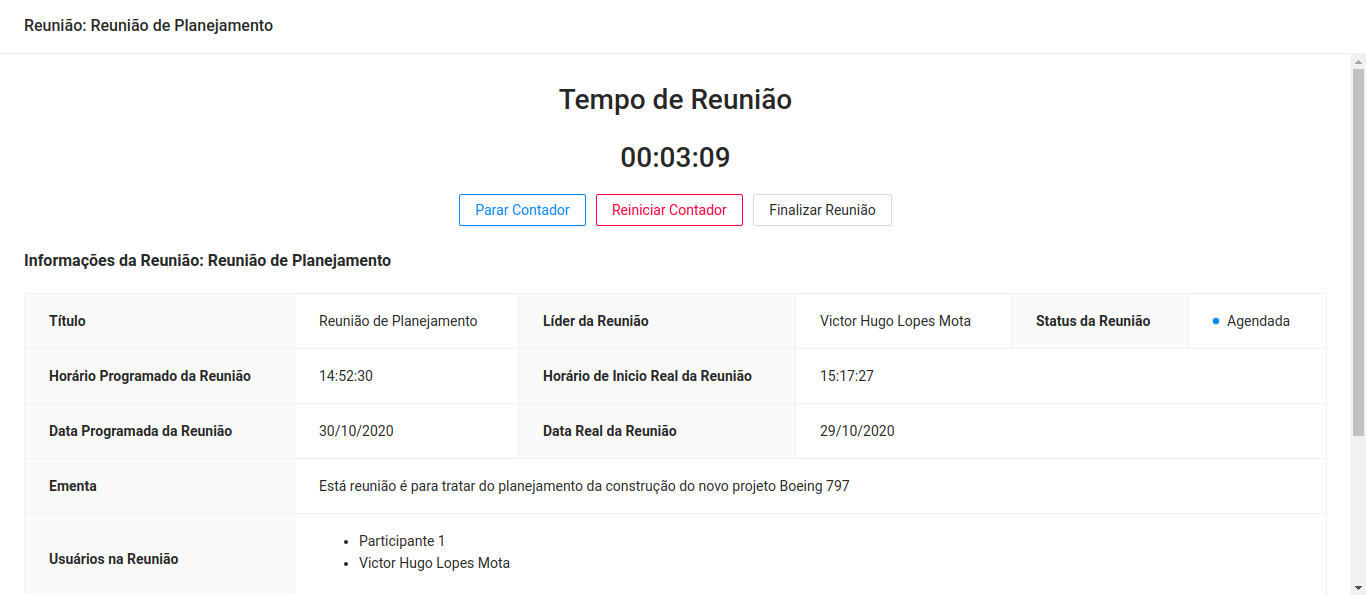
\includegraphics[width=1.0\textwidth]{figuras/informacoes_reuniao.png}
    \caption{Informações da Reunião. Fonte: Própria}
    \label{img:informacoes_reuniao}
\end{figure}

Na imagem \ref{img:informacoes_reuniao}, se tem todas as informações referentes a esta reunião, bem como quatro botões: "Começar Reunião", "Parar Contador", "Reiniciar Contador", "Finalizar Reunião".

Quando o usuário aperta o botão "Finalizar Reunião", o sistema muda o status da reunião para "Finalizada" e desbloqueando as opções "Visualizar Ata" e "Novo Questionário". 

\begin{figure}[H]
    \centering
    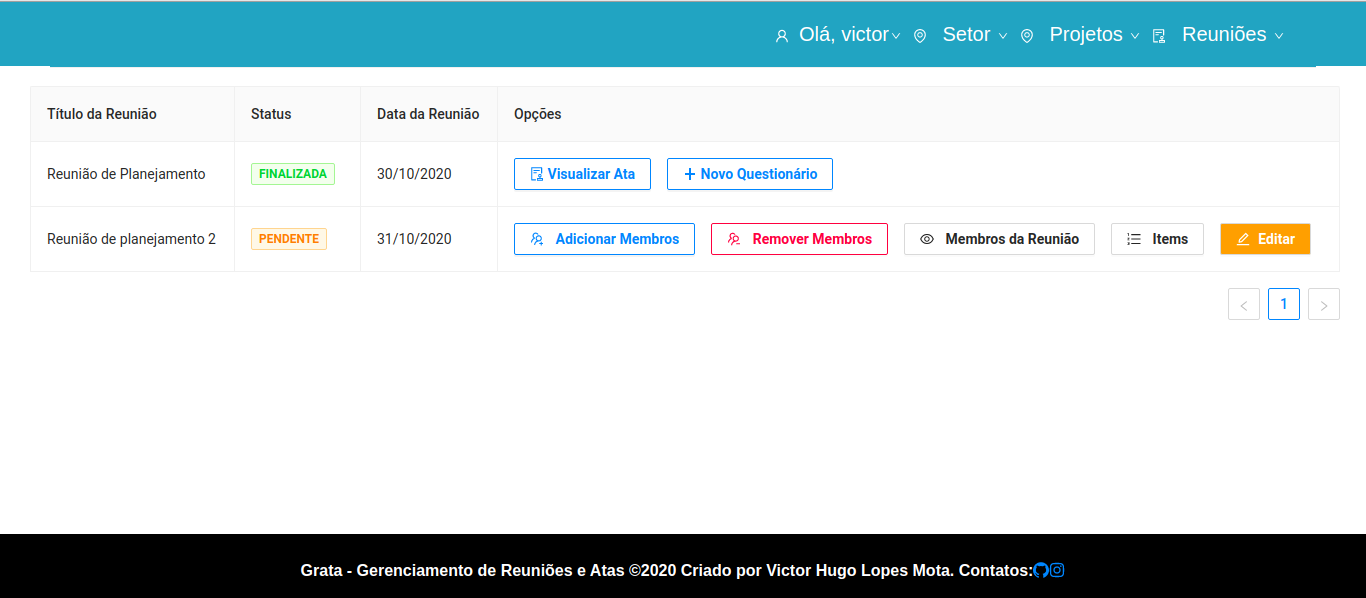
\includegraphics[width=1.0\textwidth]{figuras/reuniao_finalizada.png}
    \caption{Reunião Finalizada. Fonte: Própria}
    \label{img:reuniao_finalizada}
\end{figure}

\subsection{Visualizar Ata}

A ata de uma reunião mostra os tópicos que foram debatidos, bem como os participantes, horário de início e término da reunião. Essas informações podem ser visualizadas na imagem \ref{img:ata_reuniao}:

\begin{figure}[H]
    \centering
    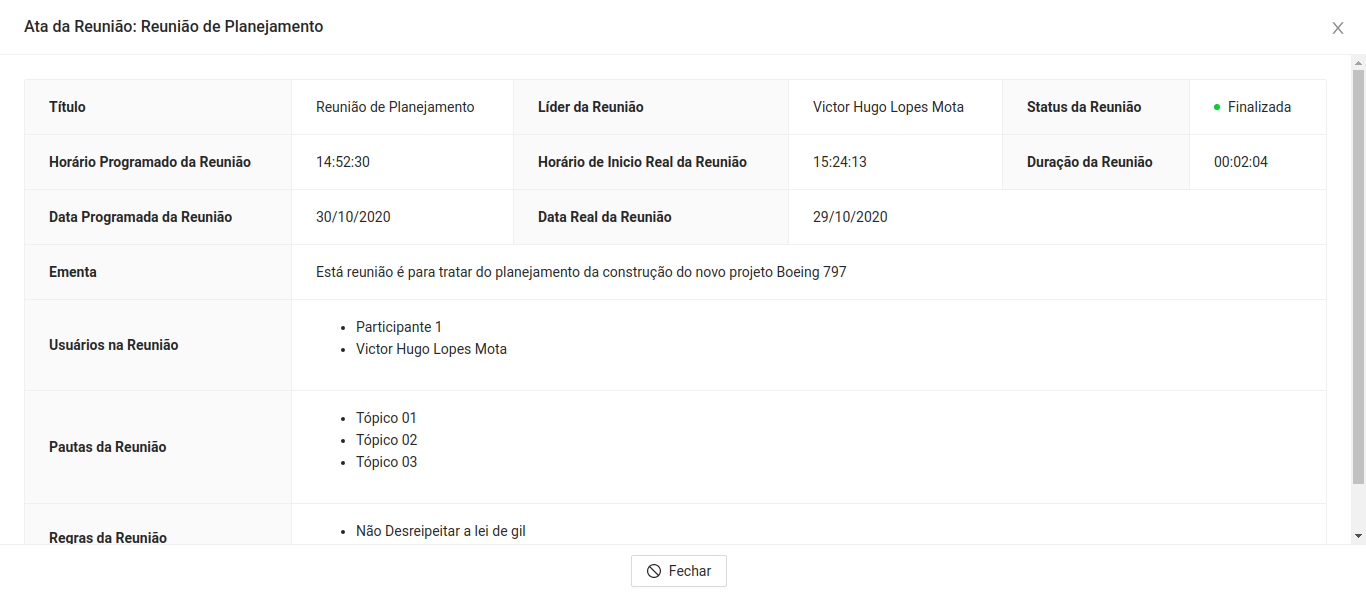
\includegraphics[width=1.0\textwidth]{figuras/visualizar_ata.png}
    \caption{Ata da Reunião. Fonte: Própria}
    \label{img:ata_reuniao}
\end{figure}

\subsection{Questionário}

O questionário possui o objetivo do gerente visualizar se os envolvidos com o projeto possuem dúvidas, e caso tenham que elas possam ser resolvidas logo. Um exemplo de questionário pode ser visto na imagem \ref{img:questionario_reuniao}:

\begin{figure}[H]
    \centering
    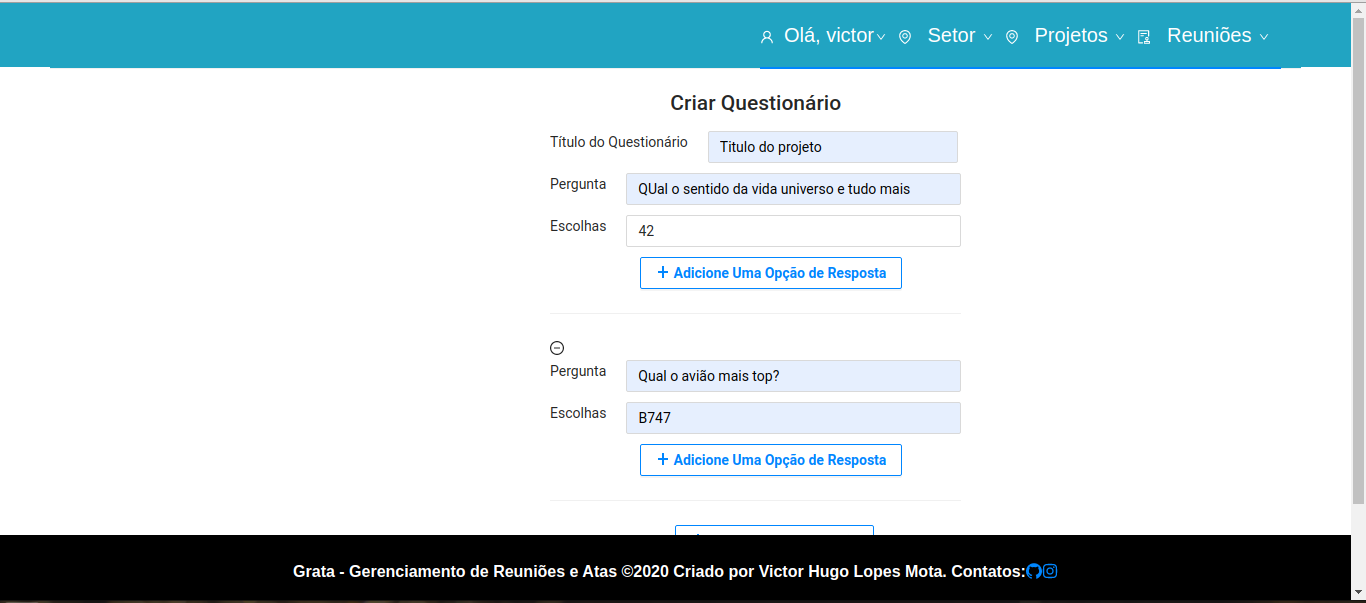
\includegraphics[width=1.0\textwidth]{figuras/questionario_reuniao.png}
    \caption{Questionário da Reunião. Fonte: Própria}
    \label{img:questionario_reuniao}
\end{figure}

\subsubsection{Responder Questionário}

Os participantes da reunião são os que podem responder os questionários, bem como ao final deste, dá uma nota para reunião. Isso faz parte do feedback dos participantes em relação a reunião ministrada pelo gerente.

\begin{figure}[H]
    \centering
    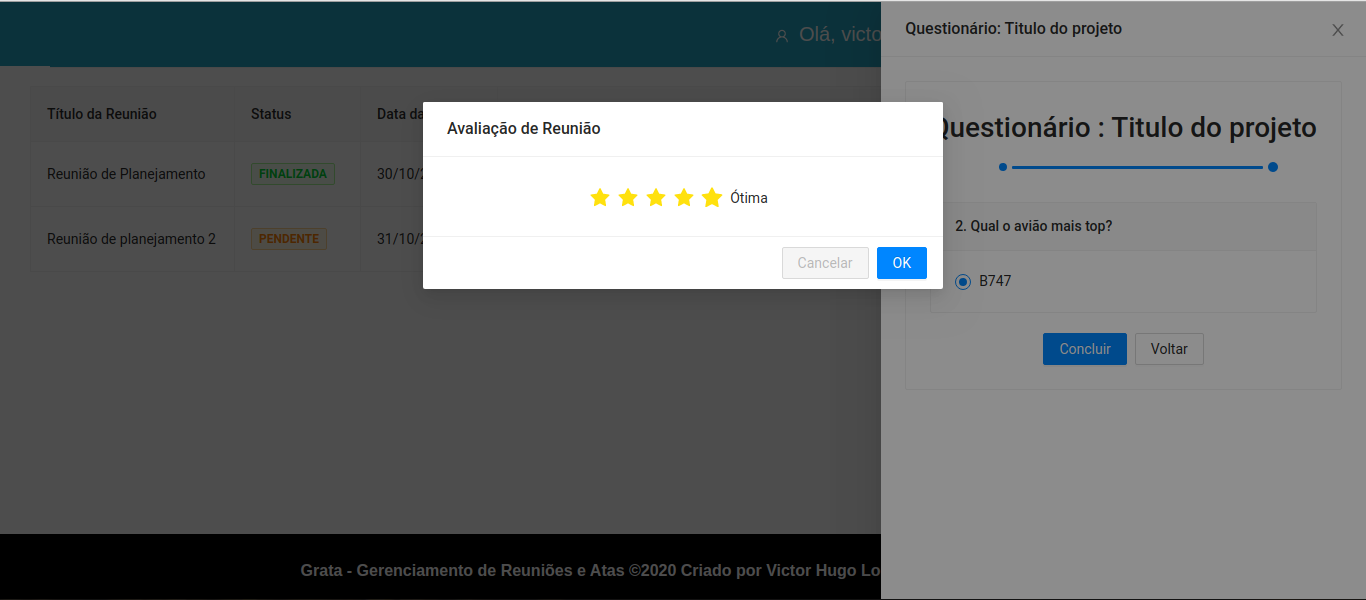
\includegraphics[width=1.0\textwidth]{figuras/avaliacao_reuniao.png}
    \caption{Avaliação da Reunião. Fonte: Própria}
    \label{img:avaliacao_reuniao}
\end{figure}

\subsection{Comentários}

Os comentários fazem parte do feedback dos participantes em relação a reunião, então é possível ao final da reunião serem colocados comentários sobre a reunião.